% documentclass: article used for scientific journals, short reports, program documentation, etc
% options: fontsize 11, generate document for double sided printing, a4-paper
\documentclass[11pt, twoside, a4paper]{article}

% package for changing page layout
\usepackage{geometry}
\geometry{a4paper, lmargin=30mm, rmargin=20mm, tmargin=30mm, bmargin=20mm}
% set indentation
\setlength{\parindent}{0mm} 

% input encoding for special characters (e.g. ä,ü,ö,ß), only for non english text
% options: utf8 as encoding standard
\usepackage[utf8]{inputenc}
% package for changing used language
% options: german or default: english
\usepackage[german]{babel}

% package for math symbols, functions and environments from ams(american mathematical society)
\usepackage{amsmath}
% package for extended symbols from ams
\usepackage{amssymb}
% package for extended symbols from stmaryrd(st mary road)
%\usepackage{stmaryrd}
% package for managing pictures
\usepackage{graphicx}

% package for some extra fonts
\usepackage{txfonts}
% package for changing color of font and paper
% options: using names of default colors (e.g red, black)
\usepackage[usenames]{color}

% package for converting eps-files to pdf-files and then include them
\usepackage{epstopdf}
% use another program (ps2pdf) for converting
% !!! important: set shell_escape=1 in /etc/texmf/texmf.cnf (Linux) for allowing to use other programs
% !!!			 or use the command line with -shell-escape
\epstopdfDeclareGraphicsRule{.eps}{pdf}{.pdf}{
ps2pdf -dEPSCrop #1 \OutputFile
}

% package for reference to last page (output number of last page)
\usepackage{lastpage}
% package for using header and footer
% options: automate terms of right and left marks
\usepackage[automark]{scrpage2}
% set style for footer and header
\pagestyle{scrheadings}
% clear pagestyle for redefining
\clearscrheadfoot
% set header and footer: use <xx>head/foot[]{Text} (i...inner, o...outer, c...center, o...odd, e...even, l...left, r...right)
\ihead[]{}
\ohead[]{}
\cfoot[]{\pagemark/\pageref{LastPage}}


% begin the document
\begin{document}
	
	\begin{figure}[h]
		\center
		% GNUPLOT: LaTeX picture with Postscript
\begingroup
  \makeatletter
  \providecommand\color[2][]{%
    \GenericError{(gnuplot) \space\space\space\@spaces}{%
      Package color not loaded in conjunction with
      terminal option `colourtext'%
    }{See the gnuplot documentation for explanation.%
    }{Either use 'blacktext' in gnuplot or load the package
      color.sty in LaTeX.}%
    \renewcommand\color[2][]{}%
  }%
  \providecommand\includegraphics[2][]{%
    \GenericError{(gnuplot) \space\space\space\@spaces}{%
      Package graphicx or graphics not loaded%
    }{See the gnuplot documentation for explanation.%
    }{The gnuplot epslatex terminal needs graphicx.sty or graphics.sty.}%
    \renewcommand\includegraphics[2][]{}%
  }%
  \providecommand\rotatebox[2]{#2}%
  \@ifundefined{ifGPcolor}{%
    \newif\ifGPcolor
    \GPcolorfalse
  }{}%
  \@ifundefined{ifGPblacktext}{%
    \newif\ifGPblacktext
    \GPblacktexttrue
  }{}%
  % define a \g@addto@macro without @ in the name:
  \let\gplgaddtomacro\g@addto@macro
  % define empty templates for all commands taking text:
  \gdef\gplbacktext{}%
  \gdef\gplfronttext{}%
  \makeatother
  \ifGPblacktext
    % no textcolor at all
    \def\colorrgb#1{}%
    \def\colorgray#1{}%
  \else
    % gray or color?
    \ifGPcolor
      \def\colorrgb#1{\color[rgb]{#1}}%
      \def\colorgray#1{\color[gray]{#1}}%
      \expandafter\def\csname LTw\endcsname{\color{white}}%
      \expandafter\def\csname LTb\endcsname{\color{black}}%
      \expandafter\def\csname LTa\endcsname{\color{black}}%
      \expandafter\def\csname LT0\endcsname{\color[rgb]{1,0,0}}%
      \expandafter\def\csname LT1\endcsname{\color[rgb]{0,1,0}}%
      \expandafter\def\csname LT2\endcsname{\color[rgb]{0,0,1}}%
      \expandafter\def\csname LT3\endcsname{\color[rgb]{1,0,1}}%
      \expandafter\def\csname LT4\endcsname{\color[rgb]{0,1,1}}%
      \expandafter\def\csname LT5\endcsname{\color[rgb]{1,1,0}}%
      \expandafter\def\csname LT6\endcsname{\color[rgb]{0,0,0}}%
      \expandafter\def\csname LT7\endcsname{\color[rgb]{1,0.3,0}}%
      \expandafter\def\csname LT8\endcsname{\color[rgb]{0.5,0.5,0.5}}%
    \else
      % gray
      \def\colorrgb#1{\color{black}}%
      \def\colorgray#1{\color[gray]{#1}}%
      \expandafter\def\csname LTw\endcsname{\color{white}}%
      \expandafter\def\csname LTb\endcsname{\color{black}}%
      \expandafter\def\csname LTa\endcsname{\color{black}}%
      \expandafter\def\csname LT0\endcsname{\color{black}}%
      \expandafter\def\csname LT1\endcsname{\color{black}}%
      \expandafter\def\csname LT2\endcsname{\color{black}}%
      \expandafter\def\csname LT3\endcsname{\color{black}}%
      \expandafter\def\csname LT4\endcsname{\color{black}}%
      \expandafter\def\csname LT5\endcsname{\color{black}}%
      \expandafter\def\csname LT6\endcsname{\color{black}}%
      \expandafter\def\csname LT7\endcsname{\color{black}}%
      \expandafter\def\csname LT8\endcsname{\color{black}}%
    \fi
  \fi
  \setlength{\unitlength}{0.0500bp}%
  \begin{picture}(8502.00,5102.00)%
    \gplgaddtomacro\gplbacktext{%
      \csname LTb\endcsname%
      \put(1078,704){\makebox(0,0)[r]{\strut{}0.000}}%
      \put(1078,1327){\makebox(0,0)[r]{\strut{}0.200}}%
      \put(1078,1950){\makebox(0,0)[r]{\strut{}0.400}}%
      \put(1078,2573){\makebox(0,0)[r]{\strut{}0.600}}%
      \put(1078,3195){\makebox(0,0)[r]{\strut{}0.800}}%
      \put(1078,3818){\makebox(0,0)[r]{\strut{}1.000}}%
      \put(1078,4441){\makebox(0,0)[r]{\strut{}1.200}}%
      \put(1210,484){\makebox(0,0){\strut{}40.0}}%
      \put(1900,484){\makebox(0,0){\strut{}50.0}}%
      \put(2589,484){\makebox(0,0){\strut{}60.0}}%
      \put(3279,484){\makebox(0,0){\strut{}70.0}}%
      \put(3968,484){\makebox(0,0){\strut{}80.0}}%
      \put(4658,484){\makebox(0,0){\strut{}90.0}}%
      \put(5347,484){\makebox(0,0){\strut{}100.0}}%
      \put(6037,484){\makebox(0,0){\strut{}110.0}}%
      \put(6726,484){\makebox(0,0){\strut{}120.0}}%
      \put(7416,484){\makebox(0,0){\strut{}130.0}}%
      \put(8105,484){\makebox(0,0){\strut{}140.0}}%
      \put(176,2572){\rotatebox{-270}{\makebox(0,0){\strut{}$U \ [V]$}}}%
      \put(4657,154){\makebox(0,0){\strut{}$\alpha \ [^\circ]$}}%
      \put(4657,4771){\makebox(0,0){\strut{}Strahlungsintensität in Abhängigkeit des Winkels}}%
    }%
    \gplgaddtomacro\gplfronttext{%
      \csname LTb\endcsname%
      \put(7118,4268){\makebox(0,0)[r]{\strut{}Messwerte}}%
    }%
    \gplbacktext
    \put(0,0){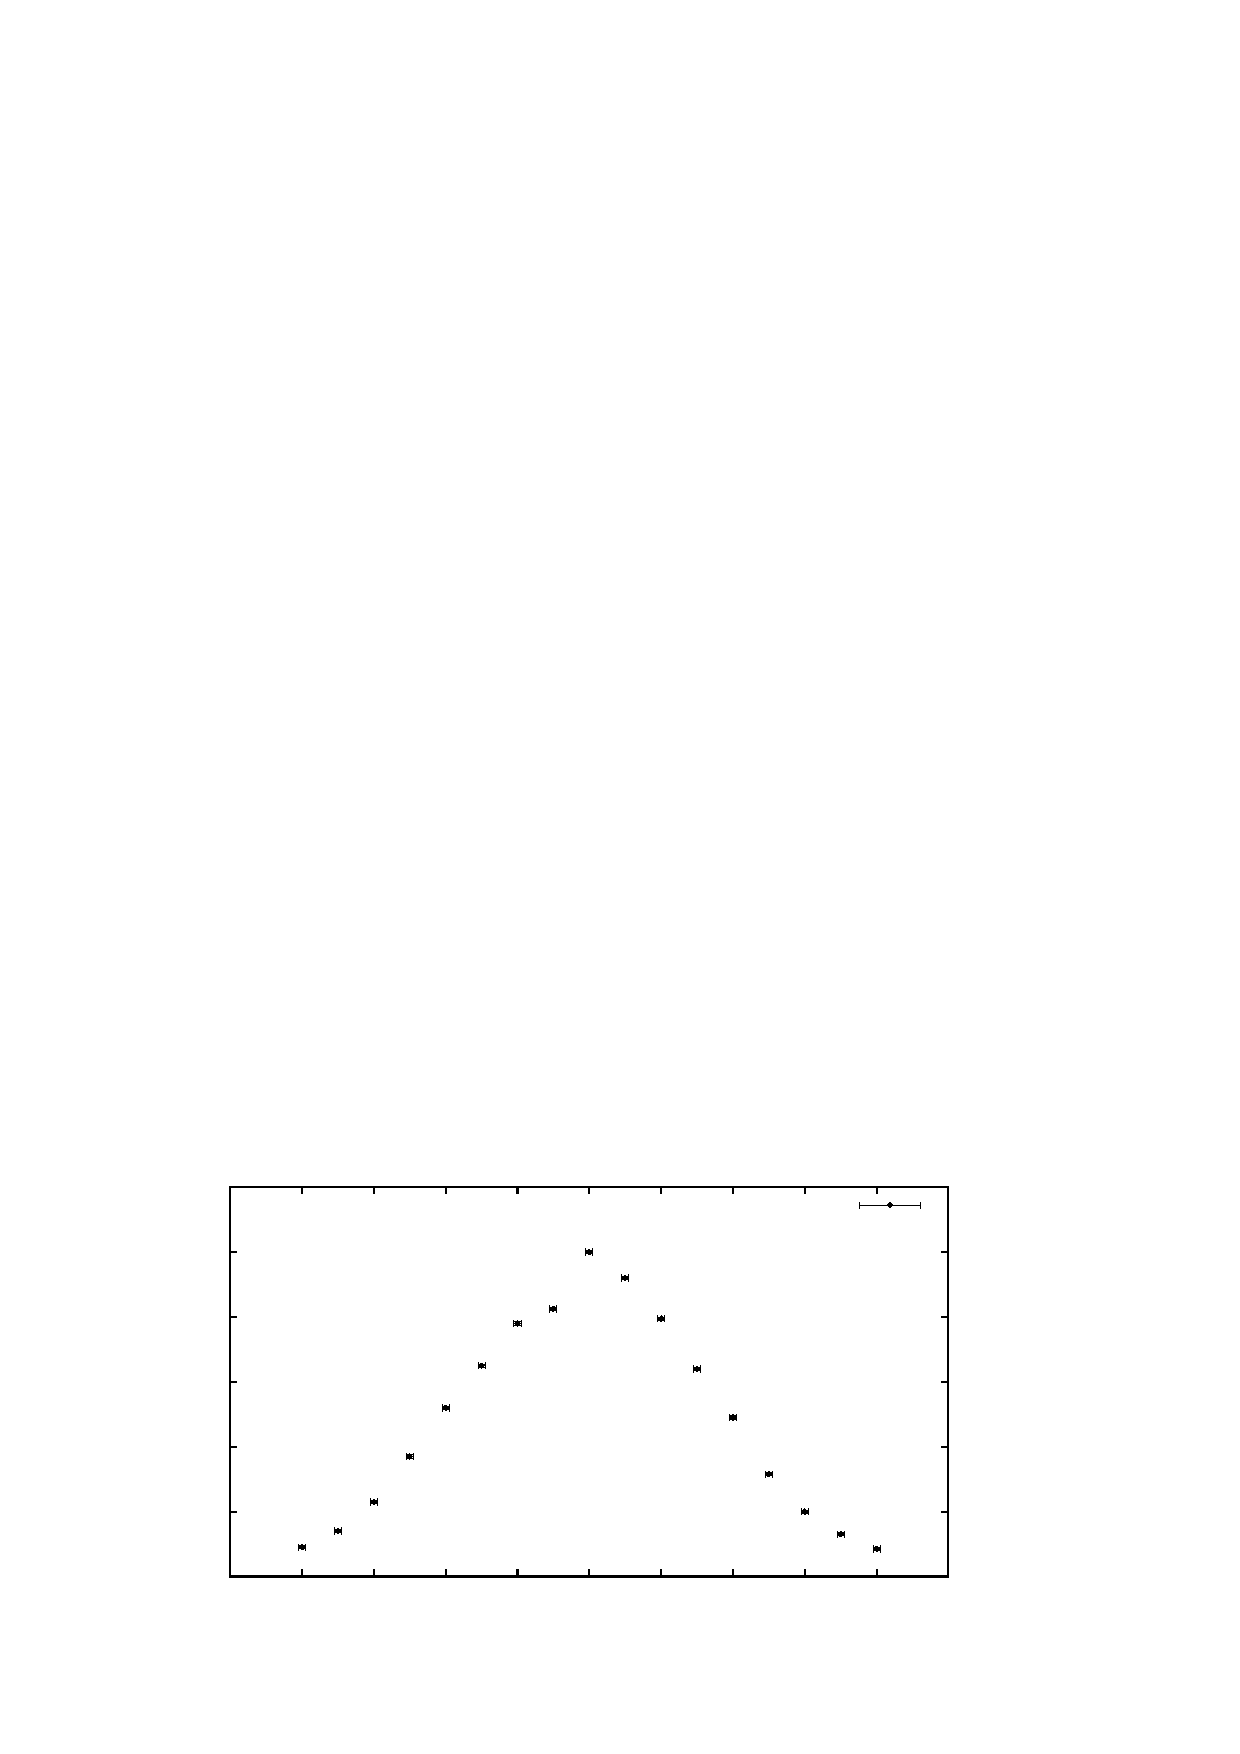
\includegraphics{u-alpha}}%
    \gplfronttext
  \end{picture}%
\endgroup

	\end{figure}

	\begin{figure}[h]
		\center
		% GNUPLOT: LaTeX picture with Postscript
\begingroup
  \makeatletter
  \providecommand\color[2][]{%
    \GenericError{(gnuplot) \space\space\space\@spaces}{%
      Package color not loaded in conjunction with
      terminal option `colourtext'%
    }{See the gnuplot documentation for explanation.%
    }{Either use 'blacktext' in gnuplot or load the package
      color.sty in LaTeX.}%
    \renewcommand\color[2][]{}%
  }%
  \providecommand\includegraphics[2][]{%
    \GenericError{(gnuplot) \space\space\space\@spaces}{%
      Package graphicx or graphics not loaded%
    }{See the gnuplot documentation for explanation.%
    }{The gnuplot epslatex terminal needs graphicx.sty or graphics.sty.}%
    \renewcommand\includegraphics[2][]{}%
  }%
  \providecommand\rotatebox[2]{#2}%
  \@ifundefined{ifGPcolor}{%
    \newif\ifGPcolor
    \GPcolorfalse
  }{}%
  \@ifundefined{ifGPblacktext}{%
    \newif\ifGPblacktext
    \GPblacktexttrue
  }{}%
  % define a \g@addto@macro without @ in the name:
  \let\gplgaddtomacro\g@addto@macro
  % define empty templates for all commands taking text:
  \gdef\gplbacktext{}%
  \gdef\gplfronttext{}%
  \makeatother
  \ifGPblacktext
    % no textcolor at all
    \def\colorrgb#1{}%
    \def\colorgray#1{}%
  \else
    % gray or color?
    \ifGPcolor
      \def\colorrgb#1{\color[rgb]{#1}}%
      \def\colorgray#1{\color[gray]{#1}}%
      \expandafter\def\csname LTw\endcsname{\color{white}}%
      \expandafter\def\csname LTb\endcsname{\color{black}}%
      \expandafter\def\csname LTa\endcsname{\color{black}}%
      \expandafter\def\csname LT0\endcsname{\color[rgb]{1,0,0}}%
      \expandafter\def\csname LT1\endcsname{\color[rgb]{0,1,0}}%
      \expandafter\def\csname LT2\endcsname{\color[rgb]{0,0,1}}%
      \expandafter\def\csname LT3\endcsname{\color[rgb]{1,0,1}}%
      \expandafter\def\csname LT4\endcsname{\color[rgb]{0,1,1}}%
      \expandafter\def\csname LT5\endcsname{\color[rgb]{1,1,0}}%
      \expandafter\def\csname LT6\endcsname{\color[rgb]{0,0,0}}%
      \expandafter\def\csname LT7\endcsname{\color[rgb]{1,0.3,0}}%
      \expandafter\def\csname LT8\endcsname{\color[rgb]{0.5,0.5,0.5}}%
    \else
      % gray
      \def\colorrgb#1{\color{black}}%
      \def\colorgray#1{\color[gray]{#1}}%
      \expandafter\def\csname LTw\endcsname{\color{white}}%
      \expandafter\def\csname LTb\endcsname{\color{black}}%
      \expandafter\def\csname LTa\endcsname{\color{black}}%
      \expandafter\def\csname LT0\endcsname{\color{black}}%
      \expandafter\def\csname LT1\endcsname{\color{black}}%
      \expandafter\def\csname LT2\endcsname{\color{black}}%
      \expandafter\def\csname LT3\endcsname{\color{black}}%
      \expandafter\def\csname LT4\endcsname{\color{black}}%
      \expandafter\def\csname LT5\endcsname{\color{black}}%
      \expandafter\def\csname LT6\endcsname{\color{black}}%
      \expandafter\def\csname LT7\endcsname{\color{black}}%
      \expandafter\def\csname LT8\endcsname{\color{black}}%
    \fi
  \fi
  \setlength{\unitlength}{0.0500bp}%
  \begin{picture}(8502.00,5102.00)%
    \gplgaddtomacro\gplbacktext{%
      \csname LTb\endcsname%
      \put(1078,704){\makebox(0,0)[r]{\strut{}0.200}}%
      \put(1078,1119){\makebox(0,0)[r]{\strut{}0.400}}%
      \put(1078,1534){\makebox(0,0)[r]{\strut{}0.600}}%
      \put(1078,1950){\makebox(0,0)[r]{\strut{}0.800}}%
      \put(1078,2365){\makebox(0,0)[r]{\strut{}1.000}}%
      \put(1078,2780){\makebox(0,0)[r]{\strut{}1.200}}%
      \put(1078,3195){\makebox(0,0)[r]{\strut{}1.400}}%
      \put(1078,3611){\makebox(0,0)[r]{\strut{}1.600}}%
      \put(1078,4026){\makebox(0,0)[r]{\strut{}1.800}}%
      \put(1078,4441){\makebox(0,0)[r]{\strut{}2.000}}%
      \put(1210,484){\makebox(0,0){\strut{}200}}%
      \put(2195,484){\makebox(0,0){\strut{}300}}%
      \put(3180,484){\makebox(0,0){\strut{}400}}%
      \put(4165,484){\makebox(0,0){\strut{}500}}%
      \put(5150,484){\makebox(0,0){\strut{}600}}%
      \put(6135,484){\makebox(0,0){\strut{}700}}%
      \put(7120,484){\makebox(0,0){\strut{}800}}%
      \put(8105,484){\makebox(0,0){\strut{}900}}%
      \put(176,2572){\rotatebox{-270}{\makebox(0,0){\strut{}$U \ [V]$}}}%
      \put(4657,154){\makebox(0,0){\strut{}$r = x_2 - x_1 \ [mm]$}}%
      \put(4657,4771){\makebox(0,0){\strut{}Strahlungsintensität in Abhängigkeit der Entfernung}}%
      \put(5938,3195){\makebox(0,0)[l]{\strut{}$a = 515552.58 \ V mm^2$}}%
      \put(5938,2780){\makebox(0,0)[l]{\strut{}$b = -271.07 \ mm$}}%
      \put(2195,4026){\makebox(0,0)[l]{\strut{}Messwerte links nicht gefittet}}%
    }%
    \gplgaddtomacro\gplfronttext{%
      \csname LTb\endcsname%
      \put(7118,4221){\makebox(0,0)[r]{\strut{}Messwerte}}%
      \csname LTb\endcsname%
      \put(7118,3906){\makebox(0,0)[r]{\strut{}$f(r) = \dfrac{a}{(r-b)^2}$}}%
    }%
    \gplbacktext
    \put(0,0){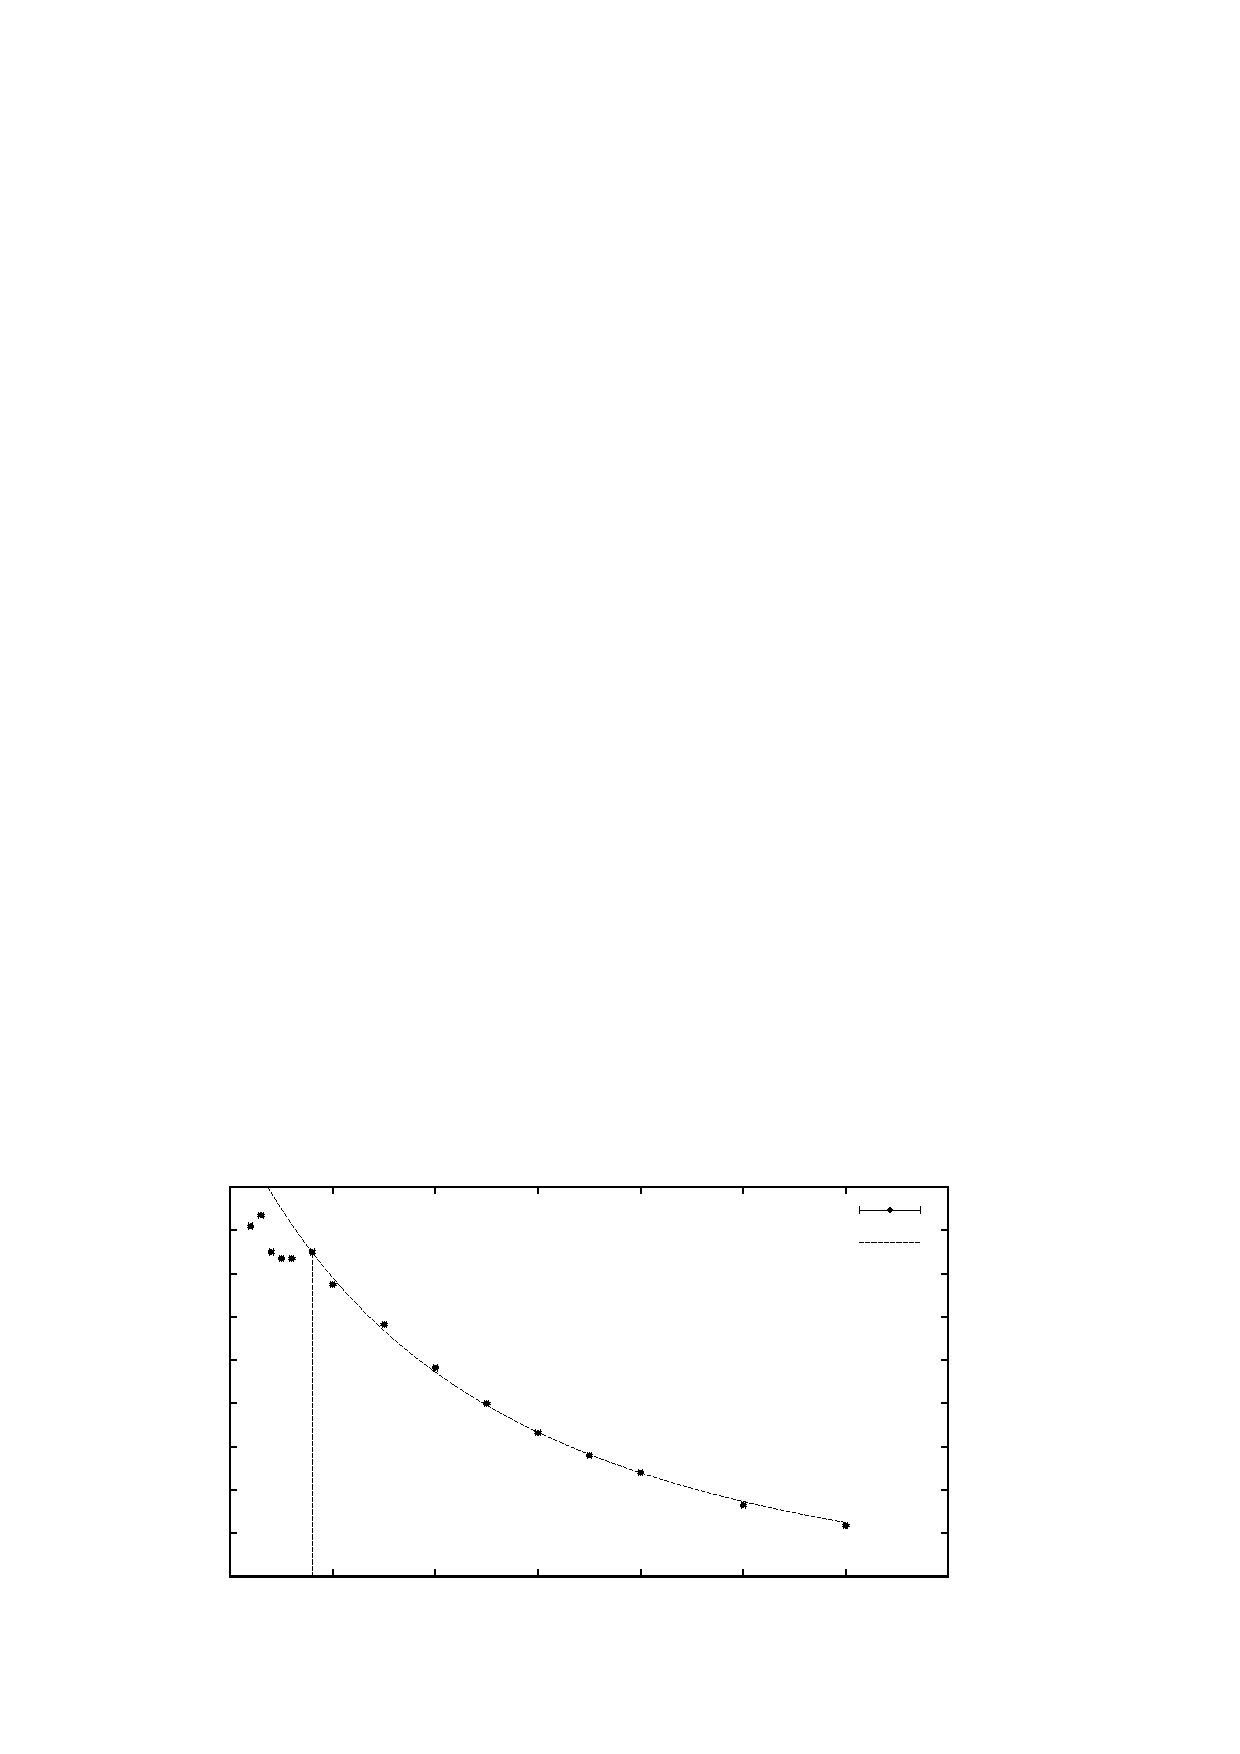
\includegraphics{u-r}}%
    \gplfronttext
  \end{picture}%
\endgroup

	\end{figure}

	\begin{figure}[h]
		\center
		% GNUPLOT: LaTeX picture with Postscript
\begingroup
  \makeatletter
  \providecommand\color[2][]{%
    \GenericError{(gnuplot) \space\space\space\@spaces}{%
      Package color not loaded in conjunction with
      terminal option `colourtext'%
    }{See the gnuplot documentation for explanation.%
    }{Either use 'blacktext' in gnuplot or load the package
      color.sty in LaTeX.}%
    \renewcommand\color[2][]{}%
  }%
  \providecommand\includegraphics[2][]{%
    \GenericError{(gnuplot) \space\space\space\@spaces}{%
      Package graphicx or graphics not loaded%
    }{See the gnuplot documentation for explanation.%
    }{The gnuplot epslatex terminal needs graphicx.sty or graphics.sty.}%
    \renewcommand\includegraphics[2][]{}%
  }%
  \providecommand\rotatebox[2]{#2}%
  \@ifundefined{ifGPcolor}{%
    \newif\ifGPcolor
    \GPcolorfalse
  }{}%
  \@ifundefined{ifGPblacktext}{%
    \newif\ifGPblacktext
    \GPblacktexttrue
  }{}%
  % define a \g@addto@macro without @ in the name:
  \let\gplgaddtomacro\g@addto@macro
  % define empty templates for all commands taking text:
  \gdef\gplbacktext{}%
  \gdef\gplfronttext{}%
  \makeatother
  \ifGPblacktext
    % no textcolor at all
    \def\colorrgb#1{}%
    \def\colorgray#1{}%
  \else
    % gray or color?
    \ifGPcolor
      \def\colorrgb#1{\color[rgb]{#1}}%
      \def\colorgray#1{\color[gray]{#1}}%
      \expandafter\def\csname LTw\endcsname{\color{white}}%
      \expandafter\def\csname LTb\endcsname{\color{black}}%
      \expandafter\def\csname LTa\endcsname{\color{black}}%
      \expandafter\def\csname LT0\endcsname{\color[rgb]{1,0,0}}%
      \expandafter\def\csname LT1\endcsname{\color[rgb]{0,1,0}}%
      \expandafter\def\csname LT2\endcsname{\color[rgb]{0,0,1}}%
      \expandafter\def\csname LT3\endcsname{\color[rgb]{1,0,1}}%
      \expandafter\def\csname LT4\endcsname{\color[rgb]{0,1,1}}%
      \expandafter\def\csname LT5\endcsname{\color[rgb]{1,1,0}}%
      \expandafter\def\csname LT6\endcsname{\color[rgb]{0,0,0}}%
      \expandafter\def\csname LT7\endcsname{\color[rgb]{1,0.3,0}}%
      \expandafter\def\csname LT8\endcsname{\color[rgb]{0.5,0.5,0.5}}%
    \else
      % gray
      \def\colorrgb#1{\color{black}}%
      \def\colorgray#1{\color[gray]{#1}}%
      \expandafter\def\csname LTw\endcsname{\color{white}}%
      \expandafter\def\csname LTb\endcsname{\color{black}}%
      \expandafter\def\csname LTa\endcsname{\color{black}}%
      \expandafter\def\csname LT0\endcsname{\color{black}}%
      \expandafter\def\csname LT1\endcsname{\color{black}}%
      \expandafter\def\csname LT2\endcsname{\color{black}}%
      \expandafter\def\csname LT3\endcsname{\color{black}}%
      \expandafter\def\csname LT4\endcsname{\color{black}}%
      \expandafter\def\csname LT5\endcsname{\color{black}}%
      \expandafter\def\csname LT6\endcsname{\color{black}}%
      \expandafter\def\csname LT7\endcsname{\color{black}}%
      \expandafter\def\csname LT8\endcsname{\color{black}}%
    \fi
  \fi
  \setlength{\unitlength}{0.0500bp}%
  \begin{picture}(8502.00,5102.00)%
    \gplgaddtomacro\gplbacktext{%
      \csname LTb\endcsname%
      \put(1078,704){\makebox(0,0)[r]{\strut{}0.000}}%
      \put(1078,1119){\makebox(0,0)[r]{\strut{}0.050}}%
      \put(1078,1534){\makebox(0,0)[r]{\strut{}0.100}}%
      \put(1078,1950){\makebox(0,0)[r]{\strut{}0.150}}%
      \put(1078,2365){\makebox(0,0)[r]{\strut{}0.200}}%
      \put(1078,2780){\makebox(0,0)[r]{\strut{}0.250}}%
      \put(1078,3195){\makebox(0,0)[r]{\strut{}0.300}}%
      \put(1078,3611){\makebox(0,0)[r]{\strut{}0.350}}%
      \put(1078,4026){\makebox(0,0)[r]{\strut{}0.400}}%
      \put(1078,4441){\makebox(0,0)[r]{\strut{}0.450}}%
      \put(1210,484){\makebox(0,0){\strut{}-5}}%
      \put(2072,484){\makebox(0,0){\strut{}0}}%
      \put(2934,484){\makebox(0,0){\strut{}5}}%
      \put(3796,484){\makebox(0,0){\strut{}10}}%
      \put(4658,484){\makebox(0,0){\strut{}15}}%
      \put(5519,484){\makebox(0,0){\strut{}20}}%
      \put(6381,484){\makebox(0,0){\strut{}25}}%
      \put(7243,484){\makebox(0,0){\strut{}30}}%
      \put(8105,484){\makebox(0,0){\strut{}35}}%
      \put(176,2572){\rotatebox{-270}{\makebox(0,0){\strut{}$U \ [V]$}}}%
      \put(4657,154){\makebox(0,0){\strut{}$d \ [mm]$}}%
      \put(4657,4771){\makebox(0,0){\strut{}Messung des Tunneleffekts und der Totalreflexion}}%
    }%
    \gplgaddtomacro\gplfronttext{%
      \csname LTb\endcsname%
      \put(7118,4268){\makebox(0,0)[r]{\strut{}Totalreflexion}}%
      \csname LTb\endcsname%
      \put(7118,4048){\makebox(0,0)[r]{\strut{}Tunneleffekt}}%
    }%
    \gplbacktext
    \put(0,0){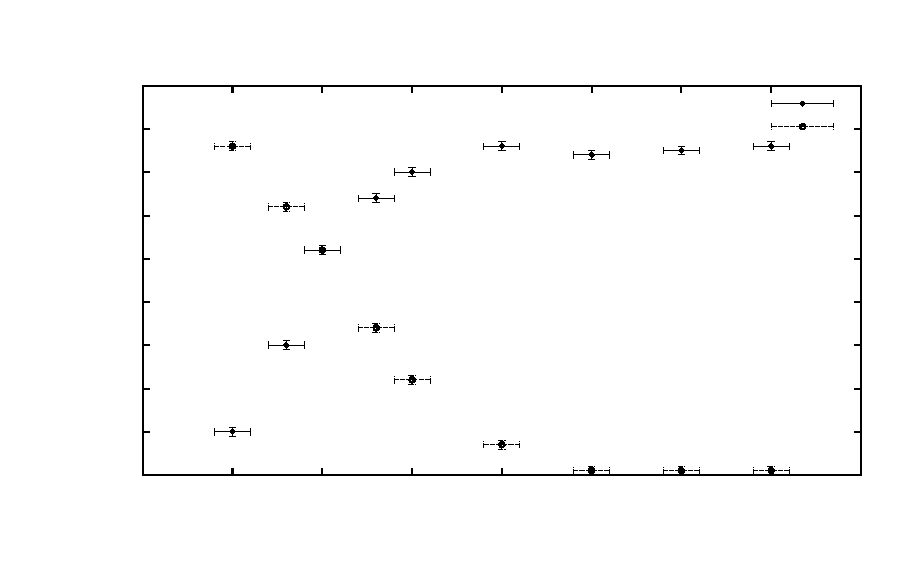
\includegraphics{u1-u2-d}}%
    \gplfronttext
  \end{picture}%
\endgroup

	\end{figure}

\end{document}

